\documentclass[14pt,aspectratio=169]{beamer}

\usepackage{pgfpages}
\usepackage{fancyvrb}

\usepackage{tikz}
\usepackage{pgfplots}

\usepackage{minted}
\usemintedstyle{tango}

\usepackage{graphicx}

\usetheme{auriga}
\usecolortheme{auriga}

\setbeamercolor{background canvas}{bg=lightgray}

% define some colors for a consistent theme across slides

\definecolor{red}{RGB}{181, 23, 0}
\definecolor{blue}{RGB}{0, 118, 186}
\definecolor{gray}{RGB}{146, 146, 146}

\title{Web Development: \\ Understanding JavaScript Fundamentals}

\author{{\bf Gregory M. Kapfhammer}}

\institute[shortinst]{{\bf Department of Computer Science, Allegheny College}}

\begin{document}

{
  \setbeamercolor{page number in head/foot}{fg=background canvas.bg}
  \begin{frame}
    \titlepage
  \end{frame}
}

% Slide
%
\begin{frame}{Technical Question}
  %
  \hspace*{.25in}
  %
  \begin{minipage}{4.75in}
    %
    \vspace*{.2in}
    %
    \begin{center}
      %
      {\large How can I leverage my understanding of the fundamentals of
        JavaScript to add interactivity and code generation to a web page by
      using functions, arrays, and objects?}
      %
    \end{center}
    %
  \end{minipage}
  %
  \vspace{3ex}
  %
  \begin{center}
    %
    \small Let's learn how to combine HTML, CSS, and JavaScript to create
    interactive web pages! Since this material assumes a knowledge of web
    pages, please review all previous content about mobile-ready web
    development! \\
    %
  \end{center}
  %
\end{frame}

% Slide
%
\begin{frame}{What is the JavaScript Programming Language?}
  %
  \begin{itemize}
    %
    \item Ullman: object-oriented, dynamically typed scripting language. What
      does each of these words mean?
      %
      \vspace*{-.15in}
      %
    \item The characteristics of the JavaScript language:
      %
      \begin{itemize}
        %
        \item {\bf Object-oriented}: almost everything in the language is an
          object
          %
        \item {\bf Dynamically typed}: you can convert the types of variables
          %
        \item {\bf Scripting language}: small scripts run on the side of the client
          %
      \end{itemize}
      %
      \vspace*{-.2in}
      %
    \item An object has both {\bf state} and {\bf behavior}
      %
      \vspace*{-.2in}
      %
    \item Variables change their types through {\bf type conversion}
      %
      \vspace*{-.2in}
      %
    \item Many argue that JavaScript is for more than scripting!
      %
  \end{itemize}
  %
\end{frame}

% Slide
%
\begin{frame}{Client-Side Scripting with JavaScript}
  %
  \begin{itemize}
    %
    \item Client-side scripting means that the JavaScript executes in the web
      browser. What are the benefits of this approach?
      %
      \vspace*{-.15in}
      %
    \item The benefits of client-side JavaScript execution:
      %
      \begin{itemize}
        %
        \item Processing can be offloaded from the server improves speed
          %
        \item Rapid response by the browser improves user experience
          %
        \item JavaScript can dynamically manipulate the HTML and CSS
          %
      \end{itemize}
      %
      \vspace*{-.2in}
      %
    \item What if the browser does not support JavaScript?
      %
      \vspace*{-.2in}
      %
    \item What if there is a defect in the JavaScript?
      %
      \vspace*{-.2in}
      %
    \item What if the web page uses too much JavaScript?
      %
  \end{itemize}
  %
\end{frame}

% Slide
%
\begin{frame}{Where Does the JavaScript Live?}
  %
  \begin{itemize}
    %
    \item The HTML source code must be able to reference the JavaScript. Where
      should we put the JavaScript?
      %
      \vspace*{-.15in}
      %
    \item The location of JavaScript in a web site:
      %
      \begin{itemize}
        %
        \item {\bf Inline}: include the JavaScript directly in the HTML
          attributes
          %
        \item {\bf Embedded}: place the JavaScript within a {\tt <script>}
          region
          %
        \item {\bf External}: place the JavaScript in files referenced by HTML
          %
      \end{itemize}
      %
      \vspace*{-.2in}
      %
    \item What are the trade-offs of these different approaches?
      %
      \vspace*{-.2in}
      %
    \item How can fail-safe design enable web accessibility?
      %
      \vspace*{-.2in}
      %
    \item What are the overall pros and cons of using JavaScript?
      %
  \end{itemize}
  %
\end{frame}

% Slide
%
\begin{frame}{Variables and Data Types in JavaScript}
  %
  \begin{itemize}
    %
      \item Variables in a JavaScript program afford the opportunity to store a
      value in a location in memory on the web client
      %
      \vspace*{-.2in}
      %
    \item Since JavaScript is dynamically typed, a variable does not have a
      declared type --- and its implicit type can change!
      %
      \vspace*{-.2in}
      %
    \item Variables in JavaScript are either {\bf reference} or {\bf primitive}
      %
      \vspace*{-.2in}
      %
    \item Examples of data types in JavaScript programs:
      %
      \begin{itemize}
        %
        \item {\bf Boolean}: stores a {\tt true} or a {\tt false} value
          %
        \item {\bf Number}: a 64-bit double-precision floating-point value
          %
        \item {\bf String}: a sequence of characters encoded in Unicode
          %
        \item {\bf Null} and {\bf Undefined}: stores no value or an undefined value
          %
      \end{itemize}
      %
      \vspace*{-.2in}
      %
  \end{itemize}
  %
\end{frame}

% Slide
%
\begin{frame}{Key Constructs of the JavaScript Language}
  %
  \begin{itemize}
    %
    \item {\bf Conditional logic} lets JavaScript take different paths
      %
      \vspace*{-.15in}
      %
    \item {\bf Iteration constructs} let JavaScript repeat and action
      %
      \vspace*{-.15in}
      %
    \item {\bf Arrays} let JavaScript store objects in a container
      %
      \vspace*{-.15in}
      %
    \item {\bf Functions} have input, produce output, and have behavior
      %
      \vspace*{-.15in}
      %
    \item {\bf Objects} contain state in variables and have behavior
      %
      \vspace*{-.15in}
      %
    \item How do these constructs work together to add a new feature? Let's
      investigate some exciting examples! Please review the text book for more
      definitions and details!
      %
      \vspace*{-.15in}
      %
  \end{itemize}
  %
\end{frame}

% Slide
%
\begin{frame}[fragile]
  \frametitle{Changing an HTML File with JavaScript}
  \normalsize
  \begin{minipage}{6in}
    \vspace*{.2in}
    \begin{minted}[mathescape, numbersep=5pt, fontsize=\large]{html}
<div class="jumbotron">
<h1><em>Hello</em> my name is
    Gregory M. Kapfhammer</h1>
<script>
document.write(randomLead());
</script>
</div>
    \end{minted}
  \end{minipage}
  %
  \vspace*{.1in}
  %
  \begin{center}
    What is the definition of the {\tt randomLead()} function?
  \end{center}
  %
\end{frame}

% Slide
%
\begin{frame}[fragile]
  \frametitle{Defining an Array of Strings in JavaScript}
  \normalsize
  \begin{minipage}{6in}
    \vspace*{.2in}
    \begin{minted}[mathescape, numbersep=5pt, fontsize=\normalsize]{javascript}
var lead = [
'<p class="lead">Oh, and I accent the
 <a href="https://github.com/AVMf/avmf">
    AVMf</a>.</p>',
'<p class="lead">Oh, and I predict with
 <a href="https://github.com/Tada-Project/tada">
    tada</a>.</p>',
];
    \end{minted}
  \end{minipage}
  %
  \vspace*{.1in}
  %
  \begin{center}
    The {\tt lead} variable is an array that contains strings of HTML!
  \end{center}
  %
\end{frame}

% Slide
%
\begin{frame}[fragile]
  \frametitle{Randomly Selecting a String from the Array}
  \normalsize
  \begin{minipage}{6in}
    \vspace*{.2in}
    \begin{minted}[mathescape, numbersep=5pt, fontsize=\large]{html}

<script type="text/javascript">
var lead = [ ... ]

function randomLead() {
   return lead[Math.floor(Math.random()
     * lead.length)];
}
</script>

    \end{minted}
  \end{minipage}
  %
\end{frame}

% Slide
%
\begin{frame}{Using JavaScript to Randomly Generate HTML}
  %
  \begin{figure}
    \centering
    
\includegraphics[scale=.085]{images/javascript-web-site.png}
    \caption{The figure's caption}
  \end{figure}
  %
\end{frame}

% Slide
%
\begin{frame}{Summary of the JavaScript with Arrays}
  %
  \begin{itemize}
    %
    \item The JavaScript was stored in an {\bf embedded} fashion
      %
      \vspace*{-.15in}
      %
    \item The {\tt lead} variable is an {\bf array} that contains strings
      %
      \vspace*{-.15in}
      %
    \item The {\tt randomLead} function selects {\bf randomly} from {\tt lead}
      %
      \vspace*{-.15in}
      %
    \item The {\tt math.random()} function generates a number
      %
      \vspace*{-.15in}
      %
    \item The {\tt document.write()} function changes the web page
      %
      \vspace*{-.15in}
      %
    \item Any questions about this example? Note that the HTML and the
      JavaScript work together to achieve a user interaction! Reload the
      page and see different content!
      %
      \vspace*{-.15in}
      %
  \end{itemize}
  %
\end{frame}

% Slide
%
\begin{frame}[fragile]
  \frametitle{Defining a Constructor for a JavaScript Object}
  \normalsize
  \begin{minipage}{6in}
    \vspace*{.2in}
    \begin{minted}[mathescape, numbersep=5pt, fontsize=\large]{javascript}
function Country(name, iso,
                 capital, population) {
  "use strict";
  this.name = name;
  this.iso = iso;
  this.capital = capital;
  this.population = population;
}
    \end{minted}
  \end{minipage}
  %
\end{frame}

% Slide
%
\begin{frame}[fragile]
  \frametitle{Creating an Array of Objects in JavaScript}
  \normalsize
  \begin{minipage}{6in}
    \vspace*{.2in}
    \begin{minted}[mathescape, numbersep=5pt, fontsize=\large]{javascript}
  var countries = [
    new Country("Bahamas", "bs",
         "Nassau", 301790),
    new Country("Canada", "ca",
         "Ottawa", 33679000),
    new Country("Germany", "de",
         "Berlin", 81802257)
  ];
    \end{minted}
  \end{minipage}
  %
\end{frame}

% Slide
%
\begin{frame}[fragile]
  \frametitle{Adding to an Array of Objects in JavaScript}
  \normalsize
  \begin{minipage}{6in}
    \vspace*{.2in}
    \begin{minted}[mathescape, numbersep=5pt, fontsize=\large]{javascript}
countries.push(new
               Country("Spain", "es",
                "Madrid", 46505963));

countries.push(new
               Country("United Kingdom", "gb",
                "London", 62348447));
    \end{minted}
  \end{minipage}
  %
\end{frame}

% Slide
%
\begin{frame}[fragile]
  \frametitle{Iterating Through an Array of Objects}
  \normalsize
  \begin{minipage}{6in}
    \vspace*{.2in}
    \begin{minted}[mathescape, numbersep=5pt, fontsize=\normalsize]{javascript}
  for (var i = 0; i < countries.length; i++) {
    var c = countries[i];
    document.write("<div class='box'>");
    document.write("<img
                     src='img/flags/" +
                     c.iso +
                     ".png'
                     class='boxImg'>");
  }
    \end{minted}
  \end{minipage}
  %
  \vspace*{.1in}
  %
  \begin{center}
    The {\tt for} loop iterates through the array and displays content!
  \end{center}
  %
\end{frame}

% Slide
%
\begin{frame}[fragile]
  \frametitle{Iterating Through the Properties of an Object}
  \normalsize
  \begin{minipage}{6in}
    \vspace*{.2in}
    \begin{minted}[mathescape, numbersep=5pt, fontsize=\normalsize]{javascript}
  for (var propertyName in c) {
    document.write("<strong>");
    document.write(propertyName + ": ");
    document.write("</strong>");
    document.write(c[propertyName]);
    document.write("<br>");
  }
    \end{minted}
  \end{minipage}
  %
  \vspace*{.1in}
  %
  \begin{center}
    The {\tt for} loop iterates through the properties of current country \\
    Using {\tt document.write} modifies the HTML of the web page \\
    What are the benefits of using JavaScript to generate HTML?
  \end{center}
  %
\end{frame}

% Slide
%
\begin{frame}{Summary of the JavaScript with Objects}
  %
  \begin{itemize}
    %
    \item The JavaScript was stored in an {\bf external} fashion
      %
      \vspace*{-.15in}
      %
    \item The {\tt countries} variable is an {\bf array} of {\tt
      Country} objects
      %
      \vspace*{-.15in}
      %
    \item The {\tt for} loop iterates through the contents of an array
      %
      \vspace*{-.15in}
      %
    \item The {\tt for} loop iterates through the contents of an object
      %
      \vspace*{-.15in}
      %
    \item The {\tt document.write()} function changes the web page
      %
      \vspace*{-.15in}
      %
    \item Any questions about this example? Note that the HTML and the
      JavaScript work together to achieve a code generation! Styling with CSS is
      also possible!
      %
      \vspace*{-.15in}
      %
  \end{itemize}
  %
\end{frame}

% Slide
%
\begin{frame}{Learn More about JavaScript}
  %
  \begin{figure}
    \centering
    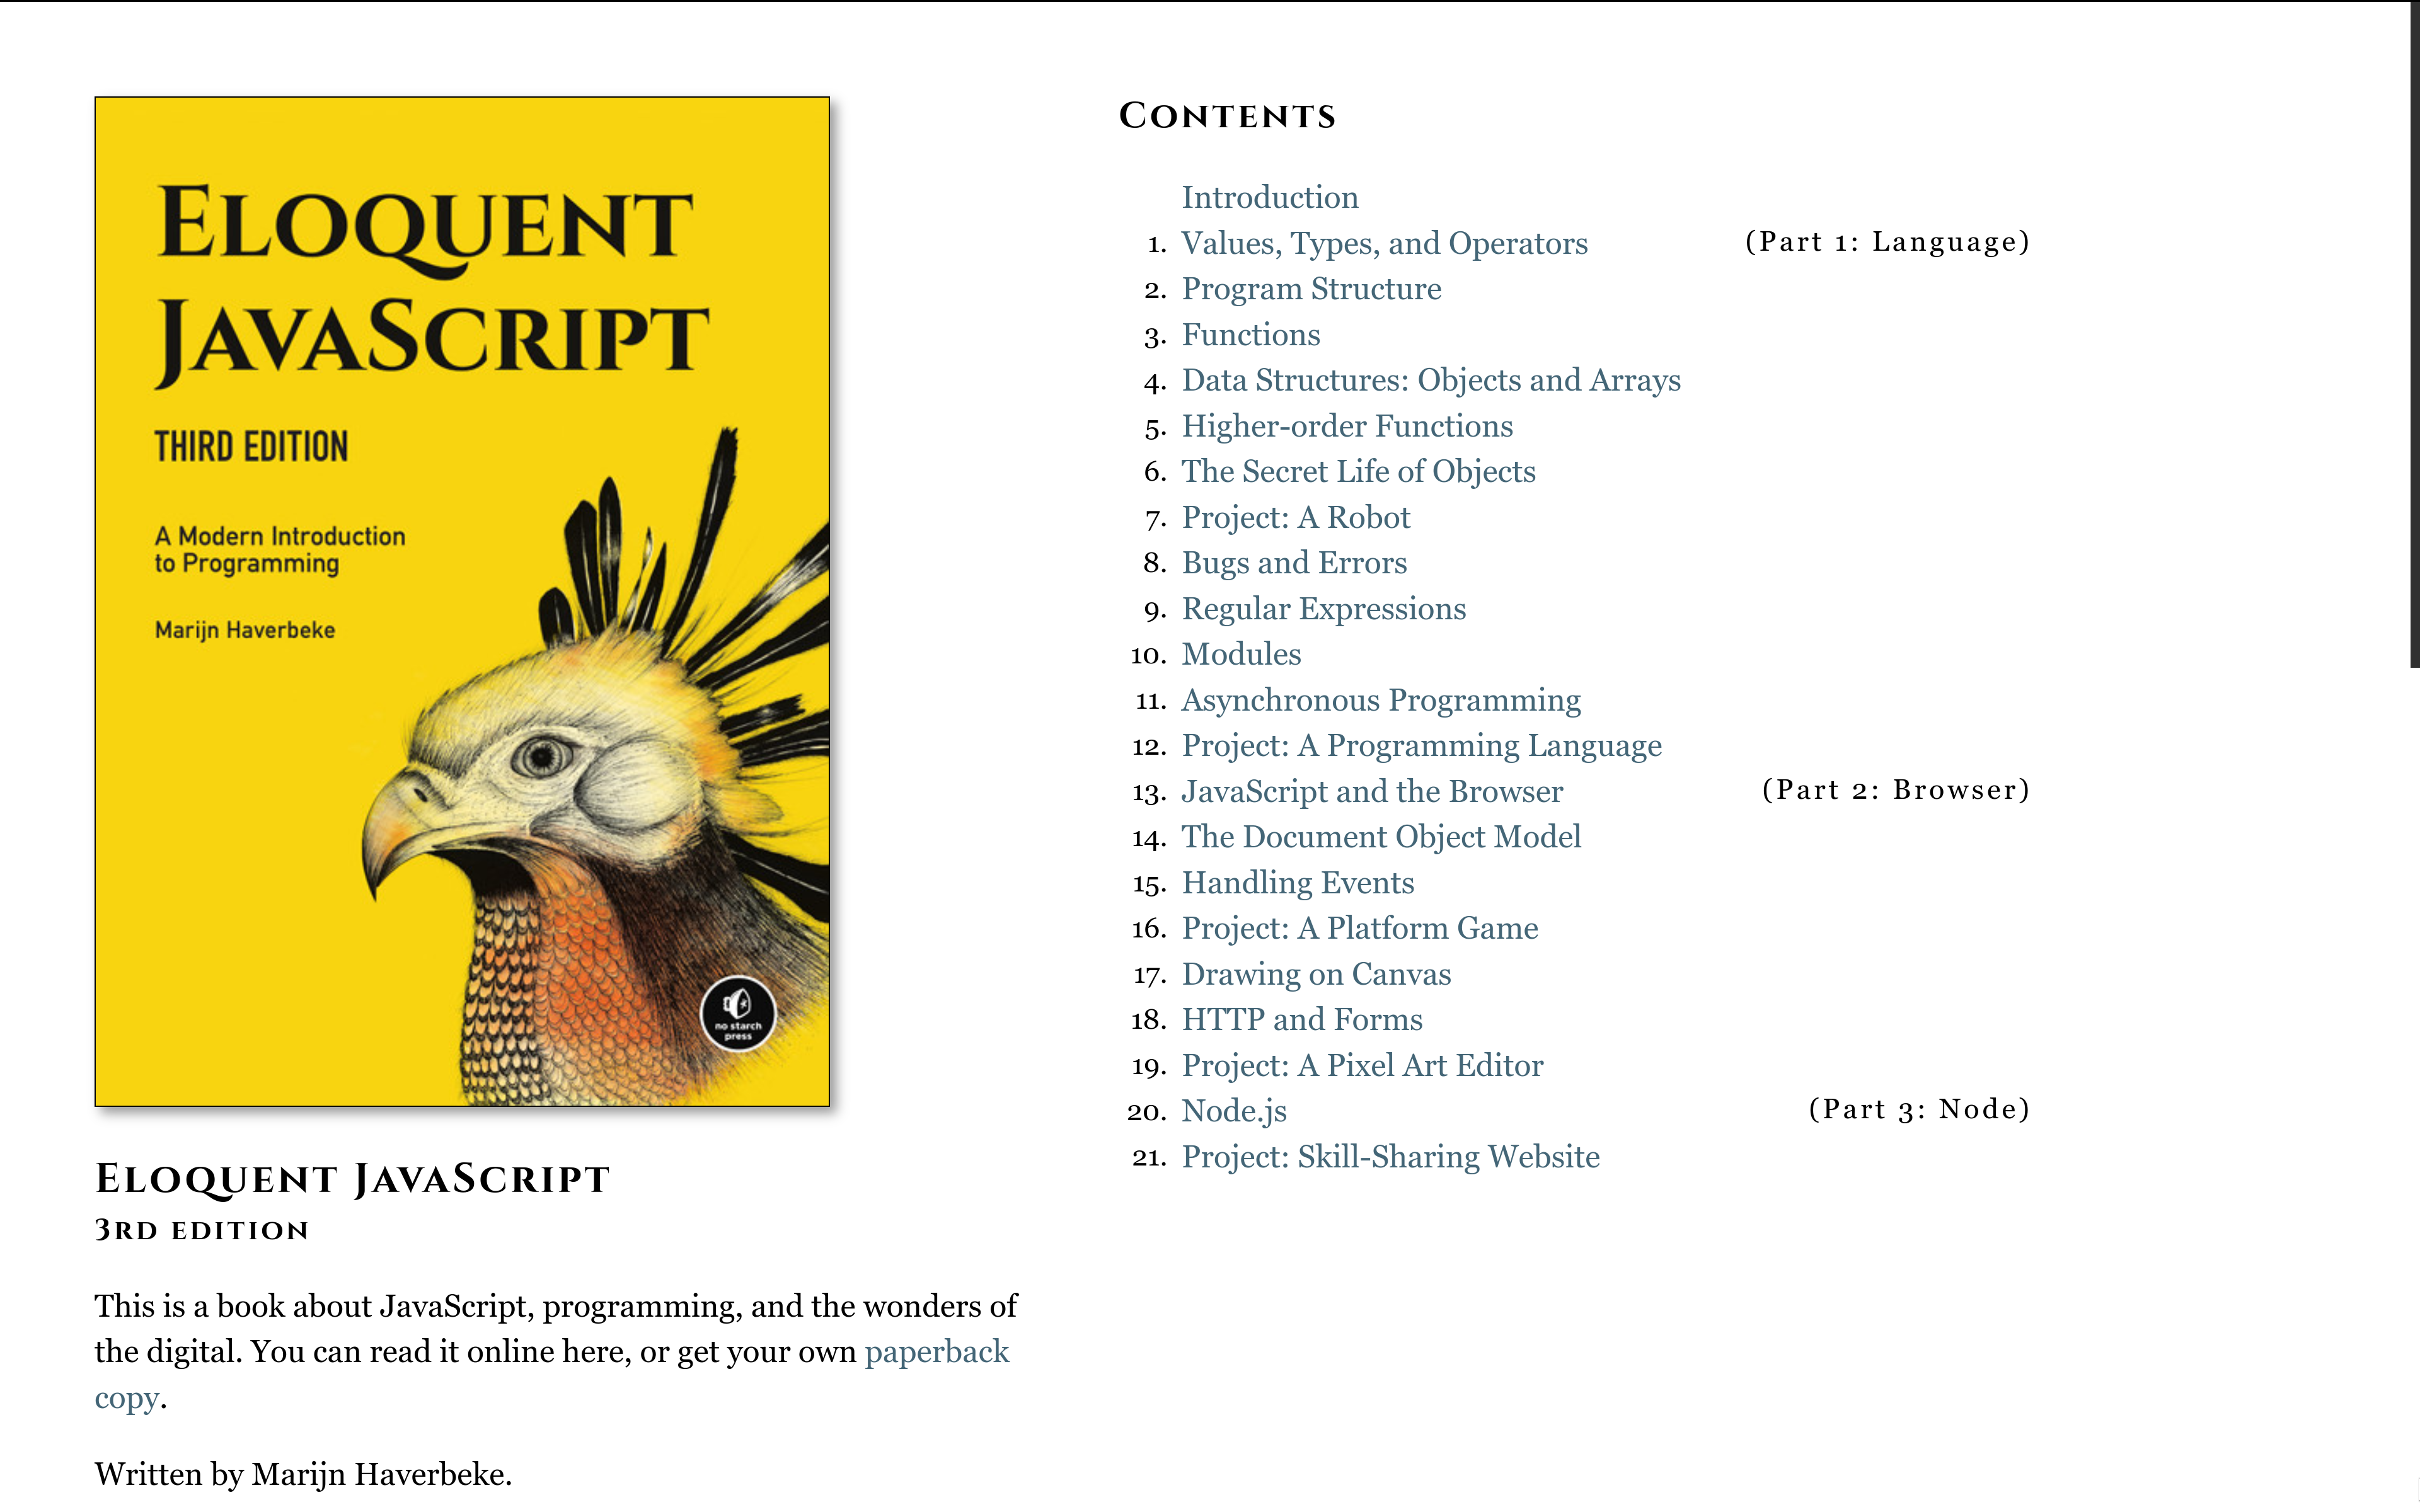
\includegraphics[scale=.085]{images/eloquent-javascript.png}
    \caption{The figure's caption}
  \end{figure}
  %
\end{frame}

% Slide
%
\begin{frame}{Learn More About JavaScript and jQuery}
  %
  \begin{figure}
    \centering
    
\includegraphics[scale=.085]{images/javascript-book.png}
    \caption{The figure's caption}
  \end{figure}
  %
\end{frame}

% Slide
%
\begin{frame}{Learn What You Don't Know About JavaScript!}
  %
  \begin{figure}
    \centering
    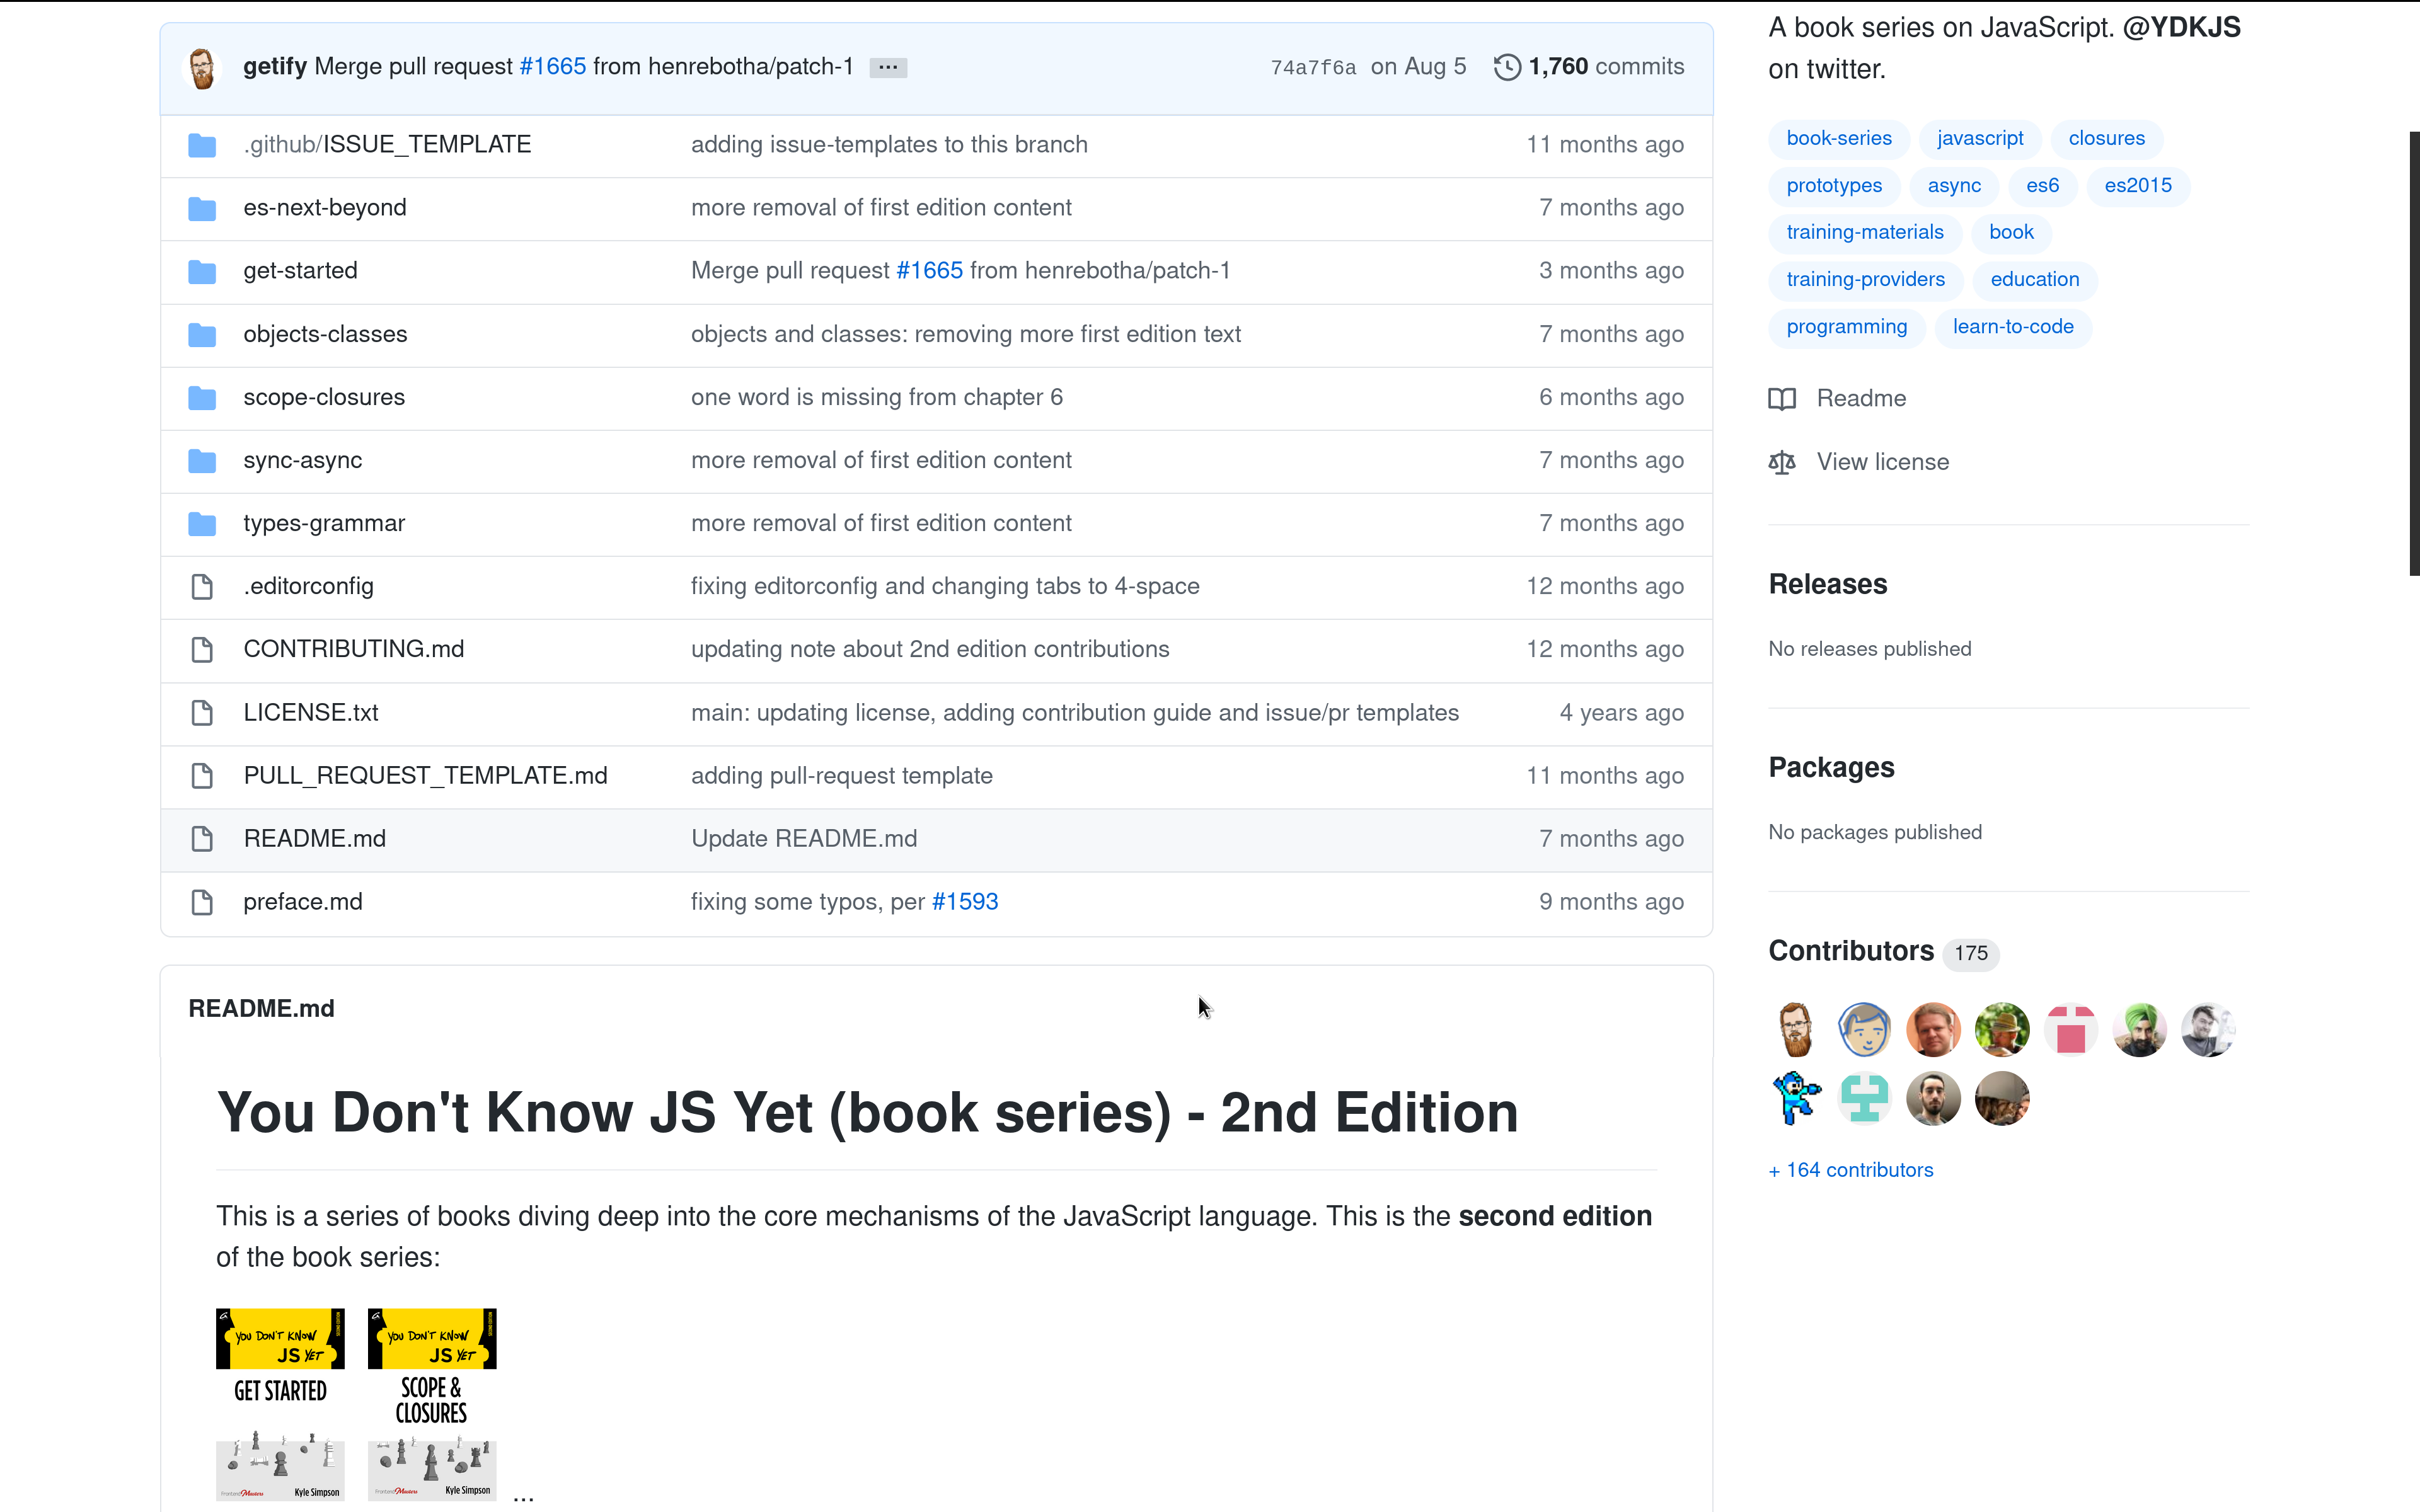
\includegraphics[scale=.085]{images/dont-know-javascript.png}
    \caption{The figure's caption}
  \end{figure}
  %
\end{frame}

\end{document}
